\documentclass[11pt]{article}
\usepackage[a4paper,margin=1in]{geometry}
\usepackage{amsmath,amssymb,amsthm,mathtools}
\usepackage{booktabs}
\usepackage{enumitem}
\usepackage{float}
\usepackage{graphicx}
\usepackage{microtype}
\usepackage{hyperref}
\usepackage[nameinlink,capitalise]{cleveref}
\usepackage[numbers,sort&compress]{natbib}

\newtheorem{theorem}{Theorem}[section]
\newtheorem{proposition}[theorem]{Proposition}
\newtheorem{corollary}[theorem]{Corollary}
\theoremstyle{definition}
\newtheorem{definition}[theorem]{Definition}
\theoremstyle{remark}
\newtheorem{remark}[theorem]{Remark}
\newcommand{\norm}[1]{\left\lVert#1\right\rVert}
\newcommand{\F}{\mathrm F}
\newcommand{\tr}{\operatorname{tr}}
\newcommand{\PhiR}{\Phi_r}

\title{Uniform Gap-Aware Quotient Laws\\
\large Price Envelopes, Stopped Safety, and a Ratio-Collapse Boundary}
\author{Liang Wang}
\date{July 2026}

\begin{document}
\maketitle

\begin{abstract}
The weak-mode quotient route has two distinct layers.  RH-96 proves a local
gap-weighted loss bound, while RH-102 proves that exact propagated debits can
be stopped against endpoint slack.  This paper supplies the missing uniform
bridge between them.

For a positive compressed block
\[
 H=\begin{pmatrix}A&C\\C^*&D\end{pmatrix},
\]
write $g=\alpha-\beta>0$ for a retained-to-omitted spectral gap and
$c=\norm C_{\F}$.  The local quotient price is
\[
 \ell=\frac{c^2}{g}.
\]
If a propagated debit is bounded by $K\ell$, then $N$ candidate quotients
fit a stopped allowance $\eta S$ whenever
\[
 N K\sup_i\frac{c_i^2}{g_i}\le\eta S.
\]
We prove that all candidates are then accepted and the endpoint gate is
preserved.  If this uniform fit fails, the same theorem gives a safe stopped
prefix: the first unaffordable candidate is rejected and the remaining chain
uses full width.  Thus uniform safety does not require a perpetual supply of
quotients.

A power corollary makes the all-level target explicit.  If
$c_i=O(\sigma^\chi\operatorname{polylog})$,
$g_i\gtrsim\sigma^\gamma/\operatorname{polylog}$,
$K=O(\sigma^{-\kappa}\operatorname{polylog})$, and the endpoint slack is
$\gtrsim\sigma^s/\operatorname{polylog}$, then the total price has signed
decay exponent $2\chi-\gamma-\kappa$.  The no-stop regime is obtained when
that exponent reaches the slack exponent $s$, with the constant budget also
fitting.  A collapsing gap is not itself an obstruction: only $c^2/g$ is
priced.

The RH-96/RH-102 audit has 38 candidate events over thresholds
$10^{-8},10^{-6},10^{-4}$.  All local gap certificates are green; the primary
five events all fit the stopped budget.  The three aggressive chains reject
three events and still preserve the endpoint gate, with worst stopped ratio
$1.006033$ versus unrestricted worst ratio $1.024921$.  The largest finite
replay-debit/local-price ratio is $0.9741$.  This closes the uniform theorem's
algebra and finite stress test, but not the physical all-level supply of gap
and cross-energy exponents.  No Stage A, Hilbert--Polya, zero identification,
or Riemann Hypothesis result is claimed.
\end{abstract}

\noindent\textbf{Keywords:} gap-aware quotient; Ky Fan loss; stopped endpoint
clock; spectral gap; adaptive Ritz enrichment; uniform price law.

\medskip
\noindent\textbf{MSC 2020:} 47A75; 15A18; 65F15; 65G20; 37C30.

\section{Introduction}

RH-95 found that a fourth projected-cross direction can be numerically
meaningless even when the corrected packet tail is stable.  RH-96 replaced
unstable direction recovery by a gap-weighted energy quotient, proving the
local estimate
\[
 \Phi_r(H)-\Phi_r(A)\le\frac{\norm C_{\F}^2}{\alpha-\beta}
 \]
under a retained-to-omitted gap \citep{WangWeakQuotient2026}.  The same paper
also showed a crucial negative result: increasing the relative cutoff can
leave every local certificate green while the recursive endpoint gate fails.

RH-102 solved the finite logical problem by assigning each proposed quotient
an exact full-suffix debit and stopping before the accumulated absolute debit
uses the endpoint slack \citep{WangStoppedClock2026}.  What remained was the
uniform question: what family-level quantity should be bounded so that a
whole candidate supply can be admitted without replaying every possible
future, and what remains safe when that supply is sparse?

The answer is a price law.  A gap is not an independent resource; it appears
only in the denominator of the quotient price $c^2/g$.  This observation has
three consequences:
\begin{enumerate}[leftmargin=2.2em]
 \item a fixed positive gap is sufficient but stronger than necessary;
 \item a collapsing gap can be harmless if the cross energy collapses faster;
 \item a stopped clock is the correct fallback when the uniform price budget
       does not fit or the candidate supply terminates.
\end{enumerate}

This paper proves those statements in one finite-dimensional theorem, derives
the sigma-power criterion, and audits the full RH-96/RH-102 data.

\section{Local gap price}
\label{sec:local}

For a positive Hermitian block matrix write
\begin{equation}
 H=\begin{pmatrix}A&C\\C^*&D\end{pmatrix}\succeq0,
 \qquad
 \Phi_r(X)=\sum_{j=1}^r\lambda_j^\downarrow(X).
 \label{eq:block}
\end{equation}
The Ky Fan variational principle is
\[
 \Phi_r(X)=\max_{P=P^*=P^2,\,\tr P=r}\tr(PX).
\]
Assume that the retained block has $\lambda_r^\downarrow(A)\ge\alpha$ and
the omitted block satisfies $D\preceq\beta I$, with
\begin{equation}
 g:=\alpha-\beta>0,
 \qquad c:=\norm C_{\F}.
 \label{eq:gap-coupling}
\end{equation}

\begin{theorem}[Local gap-weighted quotient price]
 \label{thm:local}
 Under \eqref{eq:block}--\eqref{eq:gap-coupling},
 \begin{equation}
 0\le\Phi_r(H)-\Phi_r(A)\le\ell,
 \qquad
 \ell:=\frac{c^2}{g}.
 \label{eq:local-price}
\end{equation}
\end{theorem}

\begin{proof}
 Let $P$ be a rank-$r$ projector on the full block space and write its blocks
 as $P_{ij}$.  Put $t=\tr P_{22}$.  Since
 $\tr P_{11}=r-t$ and the $r$th retained eigenvalue is at least $\alpha$,
 \[
 \tr(P_{11}A)\le\Phi_r(A)-\alpha t.
 \]
 Also $\tr(P_{22}D)\le\beta t$.  The projector identity gives
 $\norm{P_{12}}_{\F}^2\le t$.  Hence
 \[
 \tr(PH)-\Phi_r(A)
 \le-gt+2c\sqrt t
 \le\frac{c^2}{g}.
 \]
 Maximizing over $P$ proves the upper bound.  The lower bound follows by
 using projectors supported in the retained block.
\end{proof}

\begin{remark}[The priced invariant]
 The theorem does not require a stable basis for the omitted space.  It prices
 the whole weak block through the scalar ratio $c^2/g$.  A lower bound on $g$
 alone is therefore not the correct uniform target.
\end{remark}

\section{Uniform all-candidate admission and stopped safety}
\label{sec:global}

Let $R_-$ be a rigorous lower bound for a reference endpoint scale $R$, and
let $H_0^+$ be an upper bound for the all-full baseline endpoint.  For a gate
$\Gamma>1$, define the certified slack and allowance
\begin{equation}
 S=(\Gamma R_--H_0^+)_+,
 \qquad A=\eta S,
 \qquad 0\le\eta<1.
 \label{eq:slack}
\end{equation}
Suppose a candidate sequence contains $N$ local quotients.  At candidate $i$,
let $\ell_i=c_i^2/g_i$ be the local price from \cref{thm:local}, let
$d_i\ge|\delta_i|$ be a certified propagated endpoint debit, and suppose
\begin{equation}
 d_i\le K_i\ell_i.
 \label{eq:propagated-price}
\end{equation}

\begin{theorem}[Uniform gap-aware quotient law]
 \label{thm:uniform}
 Assume $S>0$, every candidate has $g_i>0$, and there are envelopes
 $K_i\le K$ and $\ell_i\le\bar\ell$.  If
 \begin{equation}
 N K\bar\ell\le A,
 \label{eq:no-stop-budget}
 \end{equation}
 then the stopped clock accepts every candidate, and the terminal endpoint
 satisfies
 \begin{equation}
 |H_N-H_0|\le NK\bar\ell\le A,
 \qquad
 H_N<\Gamma R_-le\Gamma R.
 \label{eq:no-stop-conclusion}
 \end{equation}
 If \eqref{eq:no-stop-budget} is not known, the same endpoint conclusion
 holds for the stopped prefix obtained by accepting only while the cumulative
 certified debits remain at most $A$ and switching permanently to the full
 update after the first rejection.
\end{theorem}

\begin{proof}
 For the first assertion, the cumulative debit before any candidate is at
 most $NK\bar\ell\le A$, so the admission test accepts every candidate.
 The scalar hybrid contributions telescope and the triangle inequality gives
 $|H_N-H_0|\le\sum_i d_i\le NK\bar\ell$.  Since
 $A=\eta(\Gamma R_--H_0^+)$ with $\eta<1$, the endpoint is strictly below
 $\Gamma R_-$.  For the second assertion, the same telescoping argument holds
 for the accepted prefix, while the stopping rule enforces its cumulative
 debit bound.  The later full suffix makes no further quotient debit.
\end{proof}

\begin{remark}[What is new relative to a local certificate]
 The local theorem controls $\ell_i$ at one update.  The uniform law adds the
 candidate count $N$, the propagation factor $K$, and the endpoint slack.
 These are exactly the three quantities missing from a purely local gap
 argument.  The stopped branch remains valid even when any one of them is too
 large for the no-stop inequality.
\end{remark}

\section{Sigma-power criterion}
\label{sec:powers}

The uniform law becomes a concrete all-level target after recording signed
powers.  Let $L(\sigma)$ denote a generic product of polylogarithmic factors.

\begin{theorem}[Power-priced quotient criterion]
 \label{thm:power}
 Suppose, for all sufficiently small $\sigma$, that
 \begin{align}
 N_\sigma&\le C_N L_N(\sigma),
 \label{eq:N-power}\\
 K_\sigma&\le C_K\sigma^{-\kappa}L_K(\sigma),
 \label{eq:K-power}\\
 c_{\sigma,i}&\le C_c\sigma^\chi L_c(\sigma),
 \label{eq:c-power}\\
 g_{\sigma,i}&\ge C_g\sigma^\gamma/L_g(\sigma),
 \label{eq:g-power}\\
 S_\sigma&\ge C_S\sigma^s/L_S(\sigma).
 \label{eq:S-power}
 \end{align}
 Then the total uniform price obeys
 \begin{equation}
 N_\sigma K_\sigma\sup_i\frac{c_{\sigma,i}^2}{g_{\sigma,i}}
 \le C\,\sigma^{2\chi-\gamma-\kappa}
 L_NL_KL_c^2L_g,
 \label{eq:total-power}
 \end{equation}
 for a constant $C$ depending only on the displayed constants.  If
 \begin{equation}
 2\chi-\gamma-\kappa>s,
 \label{eq:strict-power}
\end{equation}
 then the no-stop budget in \eqref{eq:no-stop-budget} holds for all
 sufficiently small $\sigma$.  At equality, it holds provided the constant
 and polylogarithmic factors fit the safety fraction.
\end{theorem}

\begin{proof}
 Square the coupling bound, divide by the gap lower bound, and multiply by
 the candidate-count and propagation envelopes.  This gives
 \eqref{eq:total-power}.  Comparing it with the slack lower bound in
 \eqref{eq:S-power} proves the strict-power assertion; equality leaves only
 the constants and logarithms.
\end{proof}

The theorem is deliberately phrased with a gap decay exponent $\gamma$ rather
than a uniform fixed gap.  It permits $g_\sigma\to0$ whenever $c_\sigma$
vanishes faster.

\begin{proposition}[Gap collapse is not the invariant]
 \label{prop:ratio}
 Let $g_\sigma=\sigma^\gamma$ and $c_\sigma=\sigma^\chi$ with $\gamma>0$.
 Then
 \begin{equation}
 \frac{c_\sigma^2}{g_\sigma}=\sigma^{2\chi-\gamma}.
 \label{eq:ratio-price}
 \end{equation}
 In particular, for $\gamma=1$, the family $c_\sigma=\sigma^{5/4}$ has
 price $\sigma^{3/2}$ even though the gap collapses, while
 $c_\sigma=\sigma^{1/2}$ has constant price one.
\end{proposition}

\begin{proof}
 Direct substitution gives \eqref{eq:ratio-price}.  The two stated cases
 have exponents $2(5/4)-1=3/2$ and $2(1/2)-1=0$.
\end{proof}

\section{Five-anchor stopped-clock audit}
\label{sec:audit}

The audit independently reads RH-96 local gap events and RH-102 stopped
hybrid chains.  The local price is recomputed as $c^2/g$ from the stored
coupling and gap bounds.  For each accepted or rejected hybrid event, the
stored propagated debit is divided by the recomputed local price to obtain a
finite replay multiplier.  This checks the three inputs to
\cref{thm:uniform}: local price, propagation price, and endpoint budget.

\begin{table}[H]
\centering
\small
\caption{Local prices and stopped endpoint outcomes over the three thresholds.}
\label{tab:audit}
\begin{tabular}{@{}lrrrrr@{}}
\toprule
threshold & candidates & accepted/rejected & min gap & max $c^2/g$ & stopped worst\\
\midrule
$10^{-8}$ & 5  & 5/0  & $2.222\,10^{-12}$ & $4.279\,10^{-13}$ & 1.001173\\
$10^{-6}$ & 11 & 10/1 & $2.189\,10^{-12}$ & $1.395\,10^{-9}$ & 1.001173\\
$10^{-4}$ & 22 & 20/2 & $2.213\,10^{-12}$ & $5.029\,10^{-8}$ & 1.006033\\
\bottomrule
\end{tabular}
\end{table}

There are 38 candidate events across the three independent threshold chains;
35 are accepted and three are rejected.  Every one of the 38 local gap
certificates is green.  The primary threshold has no rejection and uses only
$0.102\%$ of its allowance.  The largest finite replay multiplier is
$0.9741$, so the observed endpoint prices are no larger than their local
gap-price envelope on these frozen chains.

The aggressive thresholds show why the stopped branch matters.  Their
unrestricted worst endpoint/reference ratios are $1.024921$ and $1.014092$,
whereas the stopped ratios are $1.001173$ and $1.006033$.  Local validity alone
does not imply global composition, but the stopped law restores the endpoint
gate.

\begin{figure}[H]
\centering
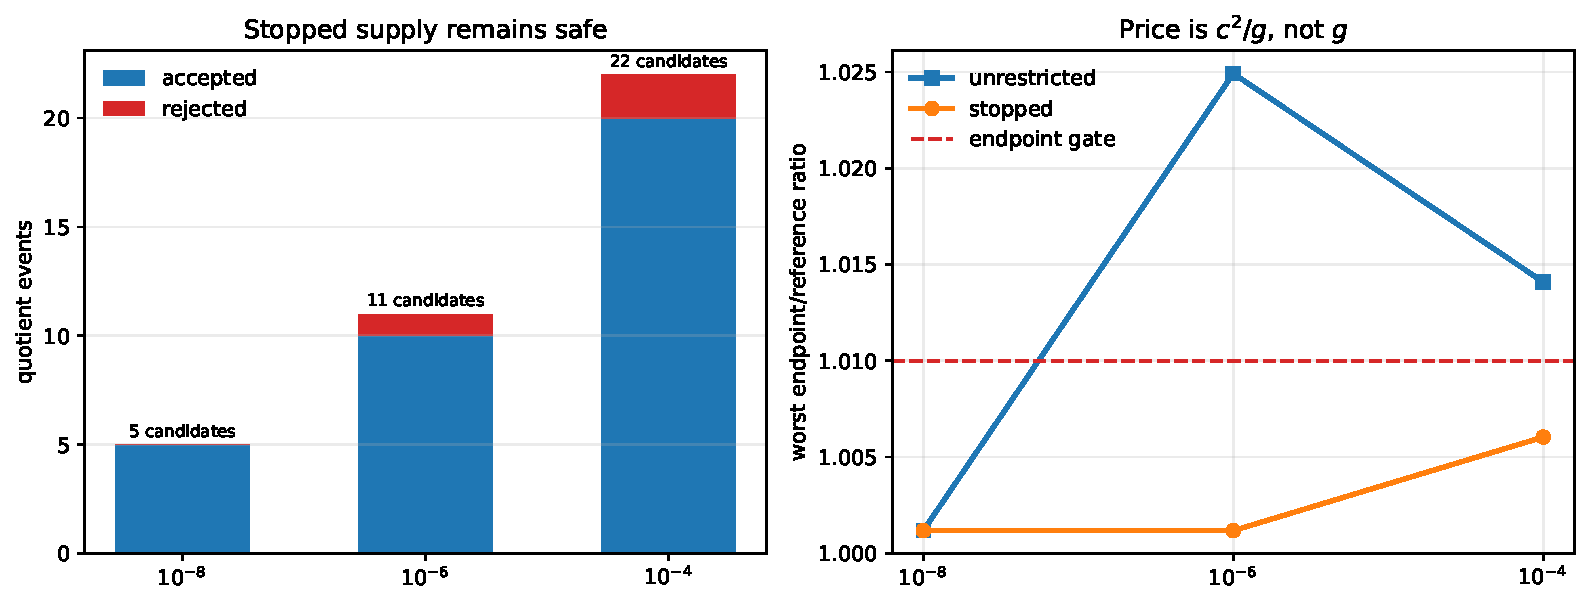
\includegraphics[width=0.98\textwidth]{figures/uniform_gap_aware_quotient.pdf}
\caption{Candidate supply and endpoint outcomes for the three thresholds.
The primary price supply fits without stopping; aggressive supplies are
truncated before the endpoint budget is exhausted.}
\label{fig:audit}
\end{figure}

For a separate ratio sanity check, the audit also evaluates the two families
in \cref{prop:ratio} at $\sigma=10^{-1},\ldots,10^{-6}$.  The good family has
price power $3/2$ despite a vanishing gap; the bad family has constant price.
This is the finite numerical signature of the power criterion, not an
estimate of the physical production exponents.

\section{Route consequence and claim boundary}
\label{sec:route}

RH-106 changes the uniform quotient question from “is there a gap?” to three
measurable conditions:
\begin{enumerate}[leftmargin=2.2em]
 \item a local price envelope $\sup c^2/g$;
 \item a propagation envelope $K$ and candidate count $N$;
 \item an endpoint slack lower bound.
\end{enumerate}
The power condition $2\chi-\gamma-\kappa\ge s$ is a sufficient no-stop
route, while the stopped theorem remains valid if the inequality fails.  This
is a genuine narrowing of the all-level gate, but it is not its proof: the
physical folded-Gaussian family has not yet supplied uniform exponents
$(\chi,\gamma,\kappa,s)$ or a replay-free $K$.

The current route ledger is therefore:
\begin{itemize}[leftmargin=2.2em]
 \item RH-104 identifies the exact physical finite-prefix target;
 \item RH-105 closes signed observation--residual algebra;
 \item RH-106 closes the abstract uniform price/stopped-safety law;
 \item physical prefix, residual, upstream, and quotient exponents remain
       open all-level inputs.
\end{itemize}

No statement here constructs a Hilbert--Polya operator, proves a $T\log T$
law or prime-power trace formula, identifies zeta zeros, or proves the
Riemann Hypothesis.

\section{Reproducibility}

The directory contains the quotient-price helpers, full and smoke audits,
figures, tests, and a hash-checked archive.  Run:
\begin{verbatim}
PYTHONDONTWRITEBYTECODE=1 /root/math/.venv/bin/python \\
  experiments/build_quotient_audit.py
PYTHONDONTWRITEBYTECODE=1 /root/math/.venv/bin/python \\
  experiments/build_quotient_audit.py --smoke
MPLBACKEND=Agg PYTHONDONTWRITEBYTECODE=1 /root/math/.venv/bin/python \\
  experiments/make_figures.py
PYTHONDONTWRITEBYTECODE=1 /root/math/.venv/bin/pytest -q -p no:cacheprovider
\end{verbatim}
The archive scripts record the exact RH-96/RH-102 inputs and verify all
publication hashes.

\bibliographystyle{plainnat}
\bibliography{references}

\end{document}
